\documentclass[10pt,a4paper]{article}
\usepackage{color}
\usepackage{url}
\usepackage{enumitem}
\usepackage{graphicx}
\usepackage{listings}
\usepackage{verbatim}
\usepackage{array}
\usepackage{caption}
\usepackage[utf8]{inputenc}
\usepackage{pdfpages}

\author{Patrick de Niet, Joseph Hill and Florian Ecard}
    
\title{\LaTeX}
    
\begin{document}
    
\begin{figure}[t]
\centering

\includegraphics[width=7.6cm]{uva.jpg}\\
\caption{UvA logo: http://www.uva.nl/home}
\label{UvA}
\end{figure}
\maketitle


\newpage
\section{Introduction}
\paragraph{}


\newpage
\tableofcontents


\newpage
\section{Homework1}
\textbf{My image is the one added in the first page for the UvA logo \ref{UvA}}\\
\textit{I guessed it'd be nicer to have a nice introduction page :-)}

\subsection{What is a wiki?}

\paragraph{}"A federated wiki is a collection of federated wiki servers. They have the ability to share pages among one another. This kind of wiki aims to prove that if it had been implemented since the wiki creation, it would have been better.\\
This project was started in 2012 in Portland at the Indie camp \cite{floref2}."\cite{floref1}

\subsection{What is a federated wiki?}

\paragraph{}"Ward Cunningham is the wiki's inventor, he made it in 1992.
A wiki is a web application where the users can read, add, edit or delete something that was created by anyone else.\\
As Wikipedia confirms it, a wiki is best used as an encyclopedia \cite{floref3}."\cite{floref1}

\subsection{What is the difference between them?}
\paragraph{}"The biggest difference between these two is the way the information is displayed to the user. A federated wiki is much more adapted to deeper analysis and ivestigation.\\
A normal wiki (e.g. Wikipédia), the whole content of a wiki is displayed, and its included link will redirect you to a different page. On the other hand, a federated wiki displays a wiki article within a third of a page. Therefore, when clicking on a link, another third of the screen would be diplayed. Showing different links in the same screen. There are no found limits (tested only up to 5 links) of wiki pages in a federated wiki. You will just have to scroll horizontally to find the desired wiki.\\
Last but not least, a federated wiki can host content onto different servers, whereas a simple wiki would host the whole in a single server \cite{floref1}\cite{floref3}."\cite{floref1}

\paragraph{Sources}
\begin{itemize}
\item \cite{floref1}
\item \cite{floref2} 
\item \cite{floref3}
\end{itemize}


\newpage
\section{Debian packaging system}
\textit{Due to the lack of decent documentation of the homework assignments, i will be using the 'Autotools' assignment to demonstrate my \LaTeX\ \cite{patref1}skill.}The text in this section is written by Patrick de Niet.
\subsection{How does it work?}
There are two types of Debian packages:
 
\begin{itemize}
\item
\textbf{Binary packages}, which contain executables, configuration files, man/info pages, copyright information, and other documentation. These packages are distributed in a Debian-specific archive format; they are usually distinguished by having a '.deb' file extension. Binary packages can be unpacked using the Debian utility dpkg\cite{patref2}.
\item
\textbf{Source packages}, which consist of a .dsc file describing the source package (including the names of the following files), a .orig.tar.gz file that contains the original unmodified source in gzip-compressed tar format and usually a .diff.gz file that contains the Debian-specific changes to the original source. The utility dpkg-source packs and unpacks Debian source archives; details are provided in its manual page\cite{patref2}.
\end{itemize}
 
In practice, it comes down to this:
 
Source packages are simply packages which just include source code, and can generally be used on any type of machine if the code is compiled in the right way.
\\
Binary packages are ones which have been made specifically for one type of computer, or architecture. Ubuntu supports the x86 (i386 or i686), AMD64 and PPC architectures. The correct binary packages will be used automatically, so you don't have to worry about picking the right ones\cite{patref3}.
 
\subsection{How does it deal with dependencies?}
¨Programs often use some of the same files as each other. Rather than putting these files into each package, a separate package can be installed to provide them for all of the programs that need them. So, to install a program which needs one of these files, the package containing those files must also be installed. When a package depends on another in this way, it is known as a package dependency. By specifying dependencies, packages can be made smaller and simpler, and duplicates of files and programs are mostly removed.
 
When you install a program, its dependencies must be installed at the same time. Usually, most of the required dependencies will already be installed, but a few extras may be needed, too. So, when you install a package, don't be surprised if several other packages are installed too - these are just dependencies which are needed for your chosen package to function properly.¨\cite{patref3}
 
\begin{figure}[ht]
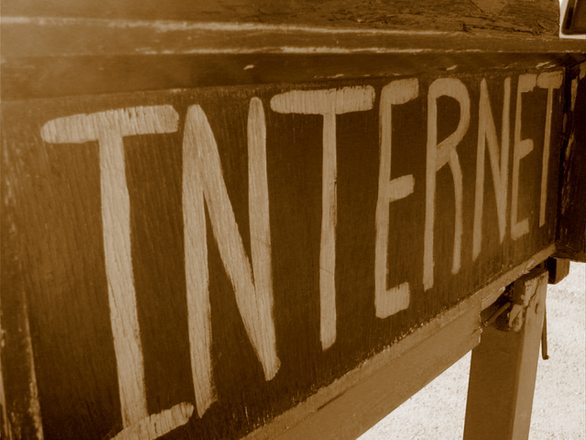
\includegraphics[width=.5in]{internet.jpg}
\caption{The (3d representation of the internet\cite{patref4})}
\end{figure}
 
\begin{table}[]
\centering
\caption{Useless table\cite{patref5}}
\label{my-label}
\begin{tabular}{lllll}
 & A  &  & B &  \\
 &  &  &  &  \\
 &  &  &  &  \\
 & C &  & D & 
\end{tabular}
\end{table}
 
 
\paragraph{Sources}
\\ 
\textcolor{red}{Summary format by Florian Ecard, continuing format for this document}
\begin{itemize}
\item \cite{patref1}
\item \cite{patref2} 
\item \cite{patref3}
\item \cite{patref4}
\item \cite{patref5}
\end{itemize}



\newpage
\section{XML in AJAX}
\subsection{What is AJAX?}
\textbf{AJAX} (Asynchronous JavaScript and XML) is a termed coined by Jesse James Garrett (figure \ref{fig:jjg}) in his article \textit{"Ajax: A New Approach to Web Applications"}\cite{JJG:AJAX}. It is a method of adding content to a webpage dynamically. Instead of linking one static page to another, the idea is to have web pages that behave more like desktop applications. Data is retrieved and added to a page without the entire page reloading. One of the first examples of this was in 1999. Internet Explorer 5 used an ActiveX control called XMLHTTP to make Outlook Web Access work more like Outlook on the desktop\cite{Wiki:XML}. This was later implemented in other browsers as the JavaScript \texttt{XMLHttpRequest} object, which was supported in Internet Explorer beginning with version 7\cite{MDN:XML}. See table \ref{tab:support} for other browsers. The \texttt{XMLHttpRequest} object allows synchronous or asynchronous requests\cite{MDN:XML}. \textbf{AJAX} specifies asynchronous requests since this prevents JavaScript from blocking while waiting for a response, allowing more responsive webpages the can continually update based on user interaction.
\begin{figure}[h]
	\centering
	
\includegraphics[width=0.2\textwidth]{jjg.jpg}
	\caption{Jesse James Garrett\cite{JJG:Photo}}
	\label{fig:jjg}
\end{figure}
\subsection{Why XML?}
Despite its name, the \texttt{XMLHttpRequest} object does not require the use of XML\cite{MDN:XML}. Other data types can be requested such as an html fragment or plain text. Without the structure and meaning provided by XML, the data retrieved is not easily understood by the clients browser. When just updating some predefined location with the data requested, this is not much of an issue. This could be used for periodically changing the advertising banner at the top of the page. However, the idea of \textbf{AJAX} is to have a much more dynamic experience. XML provides a context to the data returned that the browser can use to understand the data and make multiple changes. For instance, imagine a web based music player. As one song comes to an end the browser could make a request for the next song and receive the following XML in response.

\begin{verbatim}
<song src="/media/first.mp3">
  <title>My First Song</title>
  <artist headshot="/images/jsmith.png">John Smith</artist>
  <album year="2010" label="Big Records"
  	coverart="/images/songs.png">Songs by John Smith</album>
</song>
\end{verbatim}

The browser, now able to understand the information received, can use it to locate the media file to be played and at the same time update several different areas with information and images for the new song. One of the best examples of the power of \textbf{AJAX} is \textcolor{blue}{G}\textcolor{red}{o}\textcolor{yellow}{o}\textcolor{blue}{g}\textcolor{green}{l}\textcolor{red}{e} Maps\cite{Google:maps}. With a good internet connection, it allows the continuous scrolling of a map without any apparent loading. \texttt{XMLHttpRequest} is supported by most major browsers\cite{MDN:XML} and is a W3C draft specification\cite{W3C:XML}.
\begin{table}[h]
	\centering
	\begin{tabular}{|l|r|}
	\hline
	\textbf{Browser} & \textbf{Version}\\
	\hline
	Firefox & 1.0\\
	\hline
	Internet Explorer & 7\\
	\hline
	Safari & 1.2\\
	\hline
	Chrome & 1\\
	\hline
	\end{tabular}
	\caption{Earliest version of browsers to support \texttt{XMLHttpRequest} object\cite{MDN:XML}.}
	\label{tab:support}
\end{table}

\newpage
\listoffigures

\newpage
\bibliography{bib}{}
\bibliographystyle{plain}


\end{document}

